\documentclass{article}
\usepackage{fontspec}
\setmainfont{Libertinus Serif}
\usepackage[margin=1in]{geometry}
% Add labels to arrows
\usepackage{tikz}
\usetikzlibrary{graphs, arrows.meta}

\def\Fernandez{Fernández}
\def\Padilla{Gutiérrez de Padilla}
\def\Garcia{García de Céspedes}
\def\Vidales{Vidales}
\def\Vasquez{Vásquez}
\def\Santiago{Santiago}
\def\Lobo{Lobo}
\def\Dupont{Dupont}
\def\Jalon{Jalón}
\def\Puebla{Puebla Cathedral}
\def\Sevilla{Seville Cathedral}
\def\Malaga{Málaga Cathedral}
\def\Madrid{Madrid Royal Chapel}

\begin{document}
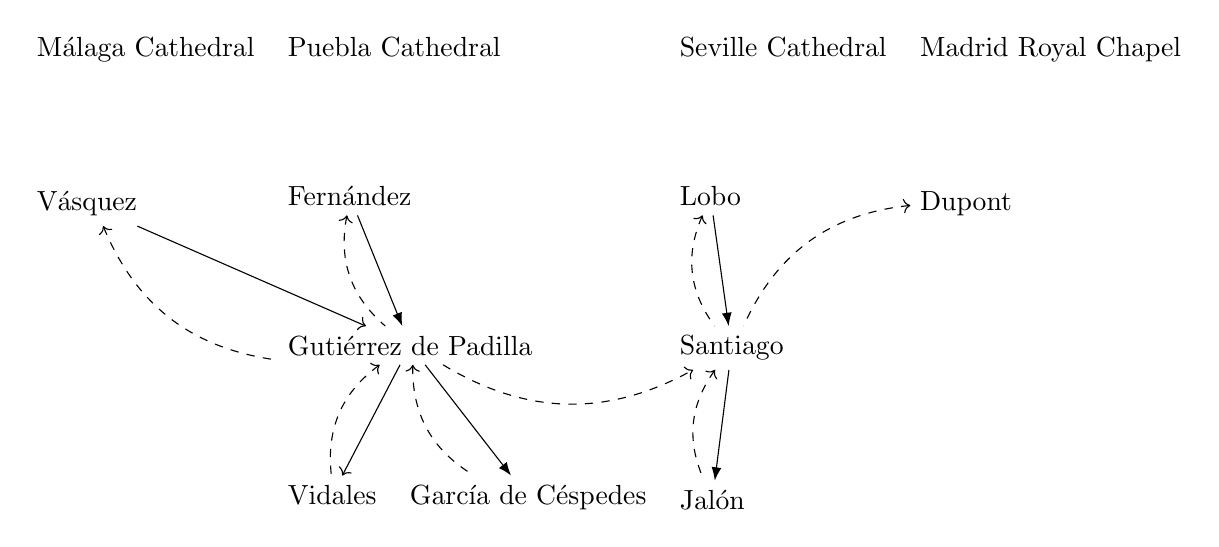
\begin{tikzpicture}
    \graph [grow down sep=4em, branch right sep=0.5em] {

    \Malaga -!- \Vasquez; 
    \Puebla -!- {
        \Fernandez <-[bend right, dashed] { 
             \Padilla <-[bend right, dashed] { \Vidales, \Garcia };
        };
        \Fernandez ->[-LaTeX] {
            \Padilla -> \Vidales;
            \Padilla ->[-LaTeX] \Garcia; 
        };
    };
    \Vasquez -> \Padilla; 
    \Sevilla -!- {
        \Lobo ->[-LaTeX] \Santiago ->[-LaTeX] \Jalon; 
        \Lobo <-[bend right, dashed] 
            \Santiago <-[bend right, dashed] 
            \Jalon;
        };
    \Madrid -!- \Dupont;
    \Dupont <-[bend right, dashed] \Santiago;
    \Padilla ->[bend right, dashed] \Santiago;
    \Vasquez <-[bend right, dashed] \Padilla;
};
\end{tikzpicture}
\end{document}

